\documentclass[12pt]{article}
\usepackage[margin=1in]{geometry}
\usepackage{setspace}\doublespacing
\usepackage{graphicx}
\usepackage{booktabs}
\usepackage{amsmath, amssymb}
\usepackage{caption}
\usepackage{subcaption}
\usepackage{hyperref}
\usepackage{float}
\usepackage{tikz}
\usetikzlibrary{arrows.meta, positioning, shapes, calc, decorations.pathreplacing}
\usepackage{pgfplots}
\pgfplotsset{compat=1.17}
\usepackage{pgfplots}
\usepackage{multirow}
\pgfplotsset{compat=newest}
\usetikzlibrary{fit, backgrounds}
% TikZ and PGFPlots for SEM diagrams and forest plots
\usepackage{tikz}
\usetikzlibrary{
  arrows.meta,
  positioning,
  shapes,
  calc,
  fit,
  backgrounds,
  decorations.pathreplacing
}
\usepackage{pgfplots}
\pgfplotsset{compat=1.18}  % or 1.17 for stability


\newcommand{\keywords}[1]{%
  \vspace{1em}
  {\noindent\textbf{Keywords:} #1}
  \vspace{1em}
}

\title{Consumer Perception Impacts on Olive Oil Consumption Choice: A Case Study Using Machine Learning Approach}
\author{Youmin Li}
\date{\today}

\begin{document}
\maketitle

\begin{abstract}
This study recognized the significance of consumer perception in shaping olive oil consumption choice. We study how consumer perceptions shape olive oil consumption choices, combining unsupervised learning for data quality and structure detection with supervised models for prediction and inference. Using exploratory factor analysis to condense multi-item perception constructs, clustering to identify respondent archetypes and remove low-quality responses, and penalized models ensembles to predict consumption preference, we quantify (i) which perceptions matter most (EFA-PCA), (ii) how effects vary across consumer segments (Cluster and SEM), and (iii) out-of-sample performance under K-fold cross-validation. Results indicate that quality perceptions, taste imagery and price sensitivity are the dominant drivers, with heterogeneity across income and region. 
\end{abstract}

\keywords{Olive oil, Consumer behavior, Agricultural food, Machine Learning}

\section{Introduction}
% Why EVOO vs ROO matters; information frictions; role of perceptions (trust, taste, price, health).
% Research gap: many correlated items; need robust prediction + interpretable drivers.
% Contributions: unified pipeline with EFA/PCA + several classes of methods + K-fold CV + ROC + importance.

Olive oil markets are increasingly differentiated by perceived quality, health benefits, origin, certification, and sensory attributes. While traditional econometric studies often examine a small set of variables, modern surveys elicit dozens of Likert-scale items and product cues that are potentially collinear and noisy. This paper leverages machine learning (ML) to: (1) reduce dimensionality and denoise multi-item perception constructs; (2) identify latent consumer segments; and (3) predict consumption outcomes.

The purpose of the paper is to reveal the impacts of consumer perception on consumption choice using choice experiment data, and olive ecological influence on consumption. So the study used factor and cluster analysis to find latent variables and incorporated consumer perception categorization into the Partial Least Squares Structural Equation Model (PLS-SEM) to explore moderation effects and mediation effects between consumer perception and consumption choice. To evaluate the prediction accuracy through cross validation. Then, the LASSO model was used to shrink corelation coefficients, and the prediction accuracy probability is greater than 90\%. This study contributes by offering an integrated pipeline that combines unsupervised learning for data curation and structure discovery with supervised learning for out-of-sample prediction and interpretable effect discovery. 


\section{Data}
% Survey context; sample size; key outcomes (binary preference; continuous consumption).
% Briefly list predictors USED AFTER EFA/PCA (factor scores + demographics).
% Refer detailed variable list, KMO/Bartlett, reliability to Appendix.

The cross-sectional data set in this paper were collected from consumers in Spain using a choice experiment and likert scale. The choice experimental questionnaire was developed through factor analysis of responses from a sample of 1031 adults. Perceived importance of olive oil attributes differs across individuals, and a five-class solution was estimated to describe each class in terms of knowledge and consumption of EVOO and the socio-demographic characteristics of the respondents. The data investigated the level of consumer awareness about the perceived health benefits, taste, price gap, and trust of EVOO and ROO by using likert scale. This information could be used to analyze consumer perceptions and preferences. Appendix table \ref{table:data} briefly describes the core subjective factor variables in the data from that questionnaire. Consumers’ trust perception and region attributes of the two olive oils are extrinsic attributes. Intrinsic attributes include perception of health benefits, taste preference, ingredient quality, and sensorial attributes. The data set source is from the Spanish Ministry of Agriculture and the University of Córdoba.

In addition, the data set includes the demographic information (age, gender, region, income, and Education level). The Table 1 shows a comparison between the sample and the population. The sample data is similar to the overall national socio-demographic background in terms of the age distribution, the gender ratio, and the distribution of education level. And the sample size of the used data set is 1031, so the study is somewhat representative of the national practical relevance of the results. 

\section{Methodology}
\subsection{Impacts pathway explanation}
The effects of mediating and moderating variables are critical concerning explaining consumer behavior, and there is a gap in previous research. To investigate the pathways linking perceptions to olive oil consumption, we estimated a partial least squares structural equation model (PLS-SEM), as shown in figure \ref{fig:1}. The model included seven reflective latent constructs: taste perception (TASTE), price perception (PRICE), health perceptions (HEALTH\_NEG), trust in extra virgin olive oil (TRUST\_EVOO), trust in refined olive oil (TRUST\_ROO), EVOO consumption (EVOO\_CONS), and ROO consumption (ROO\_CONS). Each construct was measured by multiple Likert-type items. During measurement refinement we dropped two indicators (PRICE\_2 and NEG\_CON\_2) whose standardized loadings were below the conventional 0.70 threshold (see appendix), retaining only items with strong convergent validity. We analyze individual-level survey data on olive-oil consumption in Spain with information on EVOO and ROO consumption, perceptual items for Taste, Price, Trust (split by EVOO/ROO), and a retained single Health item; demographics include gender, income group, age group, and region (e.g., Andalucía, Comunidad de Madrid). Item wording and coding follow the thesis instrument. Likert items were numeric (higher = more favorable toward EVOO); negatively phrased taste items were reverse-coded.

PLS-SEM is an approach that focuses on maximizing the explained variance in the dependent variables. It is well-suited for exploratory research or situations where theory development is in progress. It is flexible and can handle complex models with latent variables, reflective and formative indicators. And PLS-SEM focuses on estimating relationships between latent variables, which are constructed from multiple observed indicators. The estimation of the latent variables is based on the covariance structure, rather than on individual observations. This approach is less affected by heteroscedasticity at the observed level, as it accounts for measurement errors and focuses on the underlying constructs. More importantly, SEM can reveal the magnitude and direction of the effects of moderating and mediating variables. 

\begin{figure}[H]
\centering
\includegraphics[width=0.6\textwidth]{figure/sem_path_diagram.png}
\caption{SEM Path Diagram showing perception - consumption pathways.}
\label{fig:1}
\end{figure}

The final measurement model shows good reliability and validity. All retained indicators have loadings between about 0.78 and 0.95, and composite reliability (rhoC) exceeds 0.88 for all constructs (e.g., TASTE: rhoC = 0.86; TRUST\_EVOO: rhoC = 0.89; TRUST\_ROO: rhoC = 0.93; EVOO\_CONS: rhoC = 0.92; ROO\_CONS: rhoC = 0.95). Average variance extracted (AVE) is above 0.65 for every construct, indicating satisfactory convergent validity. HTMT ratios are comfortably below 0.90 for most construct pairs, supporting discriminant validity; the very high HTMT between EVOO\_CONS and ROO\_CONS reflects that many respondents consume both oils and that these two behavioral constructs are closely related rather than conceptually distinct attitudes.

The structural model was estimated with path weighting and 5000 bootstrap resamples to obtain standard errors and confidence intervals. The model explains a moderate to substantial share of the variance in the endogenous constructs: trust on EVOO and ROO. Taste perceptions significantly shape trust in both products (TASTE $\to$ TRUST\_EVOO: $\beta = -0.28$, $t \approx 9.2$; TASTE $\to$ TRUST\_ROO: $\beta = 0.19$, $t \approx 6.9$), and also have strong direct effects on consumption (TASTE $\to$ EVOO\_CONS: $\beta = -0.33$; TASTE $\to$ ROO\_CONS: $\beta = 0.33$, both $p < 0.001$). Price perceptions exert smaller but significant effects (e.g., PRICE $\to$ EVOO\_CONS: $\beta \approx 0.12$; PRICE $\to$ ROO\_CONS: $\beta \approx -0.12$). Negative health/concern perceptions strongly increase trust in ROO and slightly reduce trust in EVOO (HEALTH\_NEG $\to$ TRUST\_ROO: $\beta = 0.42$, $t \approx 15.3$; HEALTH\_NEG $\to$ TRUST\_EVOO: $\beta = -0.09$, $t \approx 3.1$), but their direct paths to consumption are small and not statistically significant.

Trust plays a central mediating role in the impact pathways from perceptions to behavior. Higher TRUST\_EVOO increases EVOO consumption and reduces ROO consumption (TRUST\_EVOO $\to$ EVOO\_CONS: $\beta = 0.33$; TRUST\_EVOO $\to$ ROO\_CONS: $\beta = -0.22$), while TRUST\_ROO has the opposite pattern (TRUST\_ROO $\to$ EVOO\_CONS: $\beta = -0.27$; TRUST\_ROO $\to$ ROO\_CONS: $\beta = 0.30$; all $p < 0.001$). The bootstrapped total effects indicate that taste and health-related concerns influence EVOO and ROO consumption both directly and indirectly through trust, confirming that trust is a key impact pathway linking perceptions to actual product choice.

After known about the impacts pathway, we adopt a two-stage approach. Stage I applies unsupervised learning to (a) clean the dataset, (b) summarize perception constructs, and (c) reveal latent consumer segments. Stage II fits supervised models, tuned via cross-validation, and evaluates predictive and structural importance. Finally, MGA compares model parameters/importance across consumer subgroups.

\subsection{Unsupervised machine learning for Structure \& Data Quality}
% factor extraction criteria; factor scores retained.
% Optional: clustering for segment checks (details in Appendix).

\subsubsection*{Factor Analysis (EFA) - PCA}
To reduce dimensionality and uncover latent constructs among the 1031 survey respondents,We apply exploratory factor analysis (EFA) using the principal component analysis method (PCA) on standardized perception items to extract low-dimensional latent constructs. We select $5$ by eigenvalue $>1$ criteria, and oblimin rotation was performed on all perception items, including trust, taste, price, and health indicators for both extra virgin (EVOO) and refined olive oil (ROO). Factor scores $\hat{\mathbf{f}}_i$ are used as inputs to supervised models. 
Sampling adequacy was high (KMO~=~0.823) and Bartlett’s test of sphericity was highly significant ($\chi^2$~=~7136.94, $p<0.001$) (table \ref{KMO}), confirming that the inter-item correlations were sufficient for factor analysis. This hybrid approach allows for a better understanding of the underlying structure of the data while reducing the dimensionality for further analysis of structural visualization. 


\begin{table}[H]
\caption{Bartlett’s test of sphericity and Kaiser–Meyer–Olkin (KMO) measure of sampling adequacy.}
\label{tab:bartlettkmo}
\centering
\begin{tabular}{@{}lcc@{}}
\toprule
\textbf{Statistic} & \textbf{Value} & \textbf{Notes} \\
\midrule
Bartlett’s test of sphericity: &  \\[2pt]
\hspace{1em}Chi-square ($\chi^{2}$) & 10{,}419.814   \\[-2pt]
\hspace{1em}Degrees of freedom & 153   \\[-2pt]
\hspace{1em}p-value & 0.000 & variables are not intercorrelated \\[4pt]
Kaiser–Meyer–Olkin (KMO) & 0.8799 & Sampling adequacy (meritorious) \\ 
\bottomrule
\end{tabular}
\label{KMO}
\end{table}


\subsubsection*{Consumer segment cluster}

Following the extraction of five latent perception factors (F1--F5), we conducted unsupervised segmentation using $k$-means clustering on the standardized factor scores. The optimal number of clusters was selected using the average silhouette coefficient. As shown in appendix figure \ref{fig:silhouette}, silhouette widths peaked at $k=5$, indicating that a five cluster solution provides the best-defined separation between consumer segments. Tthe factor-score centroids reveal five distinct perception-based consumer segments, presented in table \ref{tab:segments}. These segments differ systematically by their levels of trust (EVOO and ROO), taste valuation, price and health sensitivity, and consumption orientation. The clusters can be interpreted as in appendix \ref{tab:loadings}, and visualized in appendix figure \ref{fig:pc}. The plot highlights clear directional differences among segments, especially along the consumption polarity (PC1) and taste/trust dimensions (PC2), further confirming that these five clusters capture meaningful heterogeneity in consumer perceptions.

\begin{table}[H]
\centering
\caption{Mean standardized factor scores by perception cluster}
\begin{tabular}{lrrrrr}
\toprule
\textbf{Cluster} & \textbf{F1} & \textbf{F2} & \textbf{F3} & \textbf{F4} & \textbf{F5}\\
\midrule
1~(EVOO favor)     & $-1.35$ & $0.42$ & $-0.74$ & $0.40$ & $-1.05$\\
2~(Mild flavor) & $0.00$ & $0.09$ & $-0.30$ & $-0.83$ & $-0.45$\\
3~(Price sensitive) & $0.85$ & $0.17$ & $0.95$ & $0.03$ & $0.75$\\
4~(Taste driven)  & $0.30$ & $0.51$ & $-0.51$ & $0.75$ & $0.28$\\
5~(ROO favor) & $0.10$ & $-1.81$ & $0.83$ & $-0.37$ & $0.60$\\
\bottomrule
\end{tabular}
\label{tab:segments}
\end{table}


\subsection{Supervised machine learning}
\subsubsection{Penalized Generalized Linear Models (LASSO)}

For binary outcomes (\emph{ROO} or \emph{EVOO}), we fit LASSO-penalized logistic regression:
\begin{align}
\Pr(Y_i=1 \mid \mathbf{z}_i) &= \sigma(\beta_0 + \mathbf{z}_i^\top \boldsymbol{\beta}), \quad \sigma(t)=\frac{1}{1+e^{-t}}\\
\hat{\boldsymbol{\beta}}(\lambda) &= \arg\min_{\boldsymbol{\beta}} \left\{ -\ell(\boldsymbol{\beta}) + \lambda \|\boldsymbol{\beta}\|_1 \right\},
\end{align}
where $\mathbf{z}_i$ includes factor scores, price cues, and demographics. The L1 penalty induces sparsity, improving interpretability when many correlated inputs exist.

We fit a logistic regression with a penalty (LASSO) to predict the binary outcome of EVOO choice. The LASSO penalty performs feature selection by shrinking less-informative coefficients to zero. Using 5-fold cross-validation, we had previously identified the optimal regularization strength ($\lambda$) that minimized the mean log-loss on training folds. We fixed $\lambda$ at that value and re-trained the penalized logit model on the entire training set (80\% of data stratified by outcome). The final model was then evaluated on the 20\% hold-out test set. We assessed discrimination using the ROC AUC and accuracy at a 0.5 probability threshold, and calibration via log-loss and bias. The bias was measured as the mean predicted probability minus the actual fraction of EVOO users in the test set (ideal bias = 0 if well-calibrated). A confusion matrix was also compiled to inspect classification errors.

\subsubsection{K-fold Cross-Validation (CV).}
We tune $\lambda$ using $K=10$-fold CV. The data are partitioned into $10$ folds; each fold serves once as a validation set while the model is trained on the remaining $K-1$ folds. We select $\lambda_{\min}$ with the lowest mean validation loss (e.g., log-loss or Brier score) and optionally $\lambda_{1\mathrm{SE}}$ for a more parsimonious solution.

Overall, the results show that consumer choice between EVOO and ROO is well‐explained by a low-dimensional set of perception constructs (trust, taste, price sensitivity, health beliefs).
Importantly, even highly flexible models (RF, XGBoost, GAM) do not outperform logistic regression, indicating that the structure of the predictive relationship is largely linear and additive, with little evidence of deeper nonlinear interactions.

This provides strong evidence that the extracted perceptual factors are stable and interpretable predictors of olive‐oil choice, supporting their use for segmentation and subsequent policy or marketing analysis.


\section{Results}

\subsection{Cross-Validated Performance}
We compare models using repeated CV metrics (AUC, accuracy, log-loss for classification), calibration (reliability curves figure \ref{figure:ROC}), and fairness checks across observed subgroups. Table \ref{table:CV} reports the predictive performance of five classification models—standard logistic regression, LASSO‐penalized logistic regression, Random Forest, XGBoost boosting, and a GAM‐logit—using 10-fold cross-validation to evaluate out-of-sample performance. The model showed high discrimination (AUC = 0.91) and good accuracy (87\%). Calibration was good as indicated by a low log-loss of 0.33. The mean predicted probability of choosing EVOO was within 2\% points of the observed rate (indicating only slight bias).

\begin{table}[H]\centering
\caption{Out-of-sample performance (10-fold CV). Best in bold.}
\begin{tabular}{lcccc}
\toprule
\textbf{Model} & \textbf{ROC\_AUC} & \textbf{Accuracy} & \textbf{Log-loss} & \textbf{Notes} \\
\midrule
Logistic (baseline) & 0.90 & 0.86 & 0.33 & -- \\
LASSO-logit & \textbf{0.91} & \textbf{0.87} & \textbf{0.33} & $\lambda_{\min}$/1SE \\
Random Forest & 0.88 & 0.85 & 0.35 & 500 trees \\
Boosting & 0.88 & 0.84 & 0.35 & tuned \\
GAM-logit & 0.89 & 0.87 & 0.32 & EDF summary \\
\bottomrule
\end{tabular}
\label{table:CV}
\end{table}

% Insert combined ROC figure for binary task
\begin{figure}[H]
\centering
\includegraphics[width=0.6\linewidth]{figure/FIG_ROC_Combined.pdf}
\caption{ROC curves (10-fold CV) for the binary task: prefers EVOO (=1). 
\newline \footnotesize \textit{Note:} {Baseline:} OLS (continuous) and logistic regression (binary). {Shrinkage:} LASSO via cross-validated penalty. {Flexible Semi-parametric:} GAM with thin-plate splines/smooths for key factors (e.g., price gap, taste, trust). {Tree Ensembles:} Random forest and gradient boosting. {Validation:} Stratified $K$-fold CV ($K=10$). For classification, report AUC, accuracy, log-loss, and calibration.}
\label{figure:ROC}
\end{figure}



\subsection{LASSO-Logit regression model for prediction}

Finally, table \ref{tab:lasso_coef} displays the LASSO-selected coefficient estimates for each predictor (all features were retained at the chosen $\lambda$) along with their exponentiated odds ratios. Positive coefficients indicate higher likelihood of choosing EVOO. The LASSO-logistic model selected both perceptual and demographic predictors of EVOO choice. 
Among the perception factors, consumption polarity (F1), trust in ROO (F2), taste (F3), and trust in EVOO (F4) were retained, while the health/price factor (F5) was shrunk to zero. 
F1 and F3 show strong negative effects, indicating that ROO-oriented usage patterns and taste-driven preferences substantially reduce the likelihood of choosing EVOO. 
In contrast, trust in ROO (F1) and trust in EVOO (F2) post opposite effects on the odds of choosing EVOO, with odds ratios of 0.29 and 2.22, respectively. Demographic variables were mostly shrunk toward zero, suggesting limited predictive value once perceptions are controlled for. Income, discrete age grouping, and residence in producing areas remained in the model but with small effect sizes (OR between 1.09 and 1.18). We see that living in an olive-oil producing area is associated with increased odds of EVOO use (OR=1.18), whereas a one unit higher “Price-sensitive” factor score (Factor 3) lowers the odds (OR=0.4). Overall, the selected predictors and their odds ratios align with domain expectations.

\begin{table}[H]
\centering
\caption{LASSO-logit coefficients and odds ratios for predicting EVOO choice}
\begin{tabular}{lrr}
\toprule
\textbf{Factor} & \textbf{Coefficient ($\beta$)} & \textbf{Odds Ratio} \\
\midrule
F1: Trust in ROO & $-1.13$ & $0.29$ \\
F2: Trust in EVOO & $0.92$ & $2.22$ \\
F3: Price perception & $-0.86$ & $0.40$ \\
F4: Taste perception & $0.60$ & $1.73$ \\
F5: Health perceptiony & $0.00$ & $1.00$ \\
gender & 0 & 1\\
income &0.09 & 1.1\\
age\_discret & 0.09 &1.09\\
education &0.04 &1.04\\
region &0.17 &1.18\\
\bottomrule
\end{tabular}
\label{tab:lasso_coef}
\end{table}
\centerline{\small Positive $\beta$ increases odds of EVOO choice.}

Table \ref{tab:pred} provides the confusion matrix at the 0.5 threshold, showing that most EVOO choosers were correctly identified (only 50 of 800 were missed) while about half of non-choosers were misclassified as EVOO users. This reflects EVOO’s high prevalence and the model’s tendency to predict “1” for most cases. The confusion matrix shows that the model correctly classified 94.2\% of EVOO users (TP = 147, FN = 9) and 65.3\% of ROO users (TN = 32, FP = 17). 

\begin{table}[H]
\centering
\caption{Confusion matrix for LASSO-logit predictions (test set)}
\begin{tabular}{c|cc}
\toprule
 & \textbf{Actual ROO (0)} & \textbf{Actual EVOO (1)} \\
\midrule
\textbf{Predicted ROO (0)} & 32 & 9 \\
\textbf{Predicted EVOO (1)} & 17 & 147 \\
\bottomrule
\end{tabular}
\label{tab:pred}
\end{table}



Figure \ref{fig:predic-evoo} visualizes predicted probabilities for both the training and test sets. EVOO users (1) cluster around high predicted probabilities, whereas ROO users (0) cluster around lower predicted probabilities, with similar separation patterns in both datasets. The close correspondence between training and test distributions indicates that the LASSO-logit model generalizes well and exhibits limited overfitting. The LASSO-logistic model achieved strong predictive performance on the test set. The mean prediction bias was extremely small (Bias = --0.0024), indicating that the model's predicted probabilities are well-calibrated, consistent with the ROC--AUC of 0.91. Most mis-classification occurred among ROO users, who are underrepresented in the sample, but the model performed exceptionally well for the dominant EVOO user class.

\begin{figure}[H]
\centering
\includegraphics[width=0.6\textwidth]{figure/pred evoo.png}
\caption{LASOO-logit model predict probability on EVOO-choice.}
\label{fig:predic-evoo}
\end{figure}

\section{Discussion and Conclusions}
% Summarize gains over baseline; which perceptions matter; practical implications for labeling/targeting.
% Limitations (cross-sectional; measurement error; generalizability).
% Future work (causal messaging tests; price/assortment data; subgroup MGA).

Perception of olive oil health benefits refers to consumer understanding of the positive effects that olive oil can have on health. Olive oil is often associated with various health benefits, including its potential to reduce the risk of cardiovascular diseases, and provide anti-inflammatory and antioxidant properties (Nocella et al., 2018). People who prioritize health and trust are more likely to be aware of the health benefits associated with olive oil. They may actively seek out information about the positive effects of olive oil and incorporate it into their dietary choices. Many people believe that any kind of olive oil is a healthy food in itself compared to other foods, so the effect of health perception is not the most significant variable compared to other influencing factors. This study has considered the trade-offs not only with olive oil attributes but also with consumer perception of trust, taste, price and socio-demographic characteristics in our study. People in olive oil producing regions pay more attention to the perception of taste. Perceived trust is the primary influence factor on most consumer groups.

We provide an end-to-end ML framework linking rich perception data to olive oil consumption choices. Unsupervised steps improved data quality and interpretability via factor-based constructs and cluster-defined segments. LASSO and random forests consistently highlighted quality/safety perceptions, taste imagery, and trust in certification/origin as primary drivers, with notable heterogeneity across consumer segments documented via MGA. 

Policy and managerial implications include (i) clearer, credible labeling and certification to reduce information frictions; (ii) targeted messaging tailored to segment-specific salience (health vs.\ price vs.\ sensory); and (iii) product positioning that aligns sensory expectations with verified quality claims. Future work could integrate price/assortment data at the store level, conduct causal experiments on messaging, and examine substitution patterns among edible oils.

To improve the sales of EVOO and maintain the competitiveness of Spanish olive oil in the international market, it is important to focus on consumer taste and trust perception. The mediating effect of attitudes to EVOO on the consumption of ROO is competitive for the consumption of EVOO. Therefore, different types of olive oil should be marketed to different consumer groups with adapted marketing strategies. Accurate and effective scientific knowledge of olive oil helps raise consumers' health awareness and WTP of quality olive oil. More importantly, eco-friendly food labeling should be promoted to raise consumers' awareness of ecological services when making consumption choices.

\bibliographystyle{plain}
\bibliography{references,bib} % or your .bib file

\appendix
\section{Appendix - Additional Tables and Figures}

\begin{figure}[H]
    \centering
    \includegraphics[width=0.5\linewidth]{EFA.pdf}
    \caption{Screen Plot}
    \label{fig:screenplot}
\end{figure}


\begin{table}[H]
\caption{Factor rotation matrix from principal component extraction.}
\label{tab:rotationmatrix}
\centering
\begin{tabular}{@{}lrrrrr@{}}
\toprule
\textbf{} & \textbf{Factor 1} & \textbf{Factor 2} & \textbf{Factor 3} & \textbf{Factor 4} & \textbf{Factor 5} \\
\midrule
Factor 1 &  0.8839 &  0.6300 &  0.6981 & -0.5602 & -0.2667 \\
Factor 2 & -0.0694 &  0.6872 &  0.0250 &  0.6798 &  0.2853 \\
Factor 3 &  0.3315 & -0.3551 &  0.2712 &  0.4350 & -0.0179 \\
Factor 4 & -0.0495 & -0.0689 &  0.3182 & -0.1862 &  0.8918 \\
Factor 5 & -0.3187 &  0.0049 &  0.5807 &  0.0156 & -0.2277 \\
\bottomrule
\end{tabular}
\label{factor_rotation}
\end{table}

\begin{table}[H]
\centering
\caption{Summary of factor interpretation based on rotated loadings}
\begin{tabular}{ll}
\toprule
\textbf{Factor} & \textbf{Interpretation / Dominant items}\\
\midrule
F1 & Trust in ROO \\
F2 & Trust in EVOO \\
F3 & Price perception\\
F4 & Taste perception\\
F5 & Health perception\\
\bottomrule
\end{tabular}
\label{tab:loadings}
\end{table}

\begin{figure}[H]
    \centering
    \includegraphics[width=0.6\linewidth]{figure/PC segments.png}
    \caption{Perception‐based consumer segments (PC projection)}
    \label{fig:pc}
\end{figure}

\begin{figure}[H]
    \centering
    \includegraphics[width=0.6\linewidth]{figure/FIG_Silhouette_kmeans.pdf}
    \caption{Cluster segments silhouette}
    \label{fig:silhouette}
\end{figure}

\begin{figure}[H]
    \centering
    \begin{subfigure}{0.48\textwidth}
        \centering
        \includegraphics[width=\linewidth]{appendix/lasso importance.png}
        \caption{LASSO}
        \label{fig:roc_a}
    \end{subfigure}
    \hfill
    \begin{subfigure}{0.48\textwidth}
        \centering
        \includegraphics[width=\linewidth]{appendix/logit importance.png}
        \caption{Logit}
        \label{fig:roc_b}
    \end{subfigure}
    \caption{Permutation variable importance (LASSO / Logit)}
    \caption*{\footnotesize Note: Variable importance (permutation), partial dependence/ALE.}
    \label{fig:twofigs_sidebyside}
\end{figure}

\section{Data Archival and Code Share}

Github: \url{https://github.com/liyoumin/Machine-learning}
\begin{itemize}
  \item \textbf{Software}: R (\texttt{tidyverse}, \texttt{psych} or \texttt{EFAtools} for EFA, \texttt{glmnet} for LASSO, \texttt{rpart}/\texttt{ranger} for trees/RF, \texttt{vip}/\texttt{iml} for importance/PD/ALE), and \texttt{caret}/\texttt{tidymodels} for CV pipelines.
  \item \textbf{Cross-validation}: stratified K-fold for classification outcomes; repeated CV for stability.
\end{itemize}


\begin{table*}[h!]
\caption{Description of variables used in the olive oil consumption study.}
\label{tab:variables}
\centering
\begin{tabular}{@{}p{3cm}p{11cm}@{}}
\toprule
\textbf{Variable} & \textbf{Description} \\
\midrule
EVOO Use & Weekly uses of extra virgin olive oil (EVOO) in the household, measured as number of meal uses per week. \\
ROO Use & Weekly uses of refined olive oil (ROO) in the household, measured as number of meal uses per week. \\
EVOO Con & Monthly consumption of EVOO in the household, in liters per month per person. \\
ROO Con & Monthly consumption of ROO in the household, in liters per month per person. \\
Trust ROO1 & Your degree of trust in ROO, 1–7 Likert scale. \\
Trust ROO2 & The degree to which you need ROO, 1–7 Likert scale. \\
Trust ROO3 & The degree to which you recommend ROO, 1–7 Likert scale. \\
Trust ROO4 & The perceived quality of ROO, 1–7 Likert scale. \\
Trust EVOO1 & Your degree of trust in EVOO, 1–7 Likert scale. \\
Trust EVOO2 & The degree to which you need EVOO, 1–7 Likert scale. \\
Trust EVOO3 & The degree to which you recommend EVOO, 1–7 Likert scale. \\
Trust EVOO4 & The perceived quality of EVOO, 1–7 Likert scale. \\
Taste 1 & “EVOO is less versatile in the kitchen due to its taste” (reverse-coded), 1–7 Likert scale. \\
Taste 2 & “I prefer a mild and light-flavored olive oil” (reverse-coded), 1–7 Likert scale. \\
Taste 3 & “EVOO adds too strong a flavor for most dishes” (reverse-coded), 1–7 Likert scale. \\
Price 1 & “Extra virgin olive oil has a suitable price,” 1–7 Likert scale. \\
Price 2 & “The price gap between EVOO and ROO is small,” 1–7 Likert scale. \\
Price 3 & “Considering annual food outlay, EVOO is a cheap product,” 1–7 Likert scale. \\
Price 4 & “Considering its features, ROO has a high price,” 1–7 Likert scale. \\
Health 1 & “EVOO and ROO have the same health benefits,” 1–7 Likert scale. \\
Health 2 & “EVOO is not as good for frying as ROO,” 1–7 Likert scale. \\
Health 3 & “EVOO and ROO have the same features except for taste,” 1–7 Likert scale. \\
\bottomrule
\end{tabular}
\label{table:data}
\end{table*}



\section{Additional information for PLS-SEM}

\begin{figure}[H]
\centering
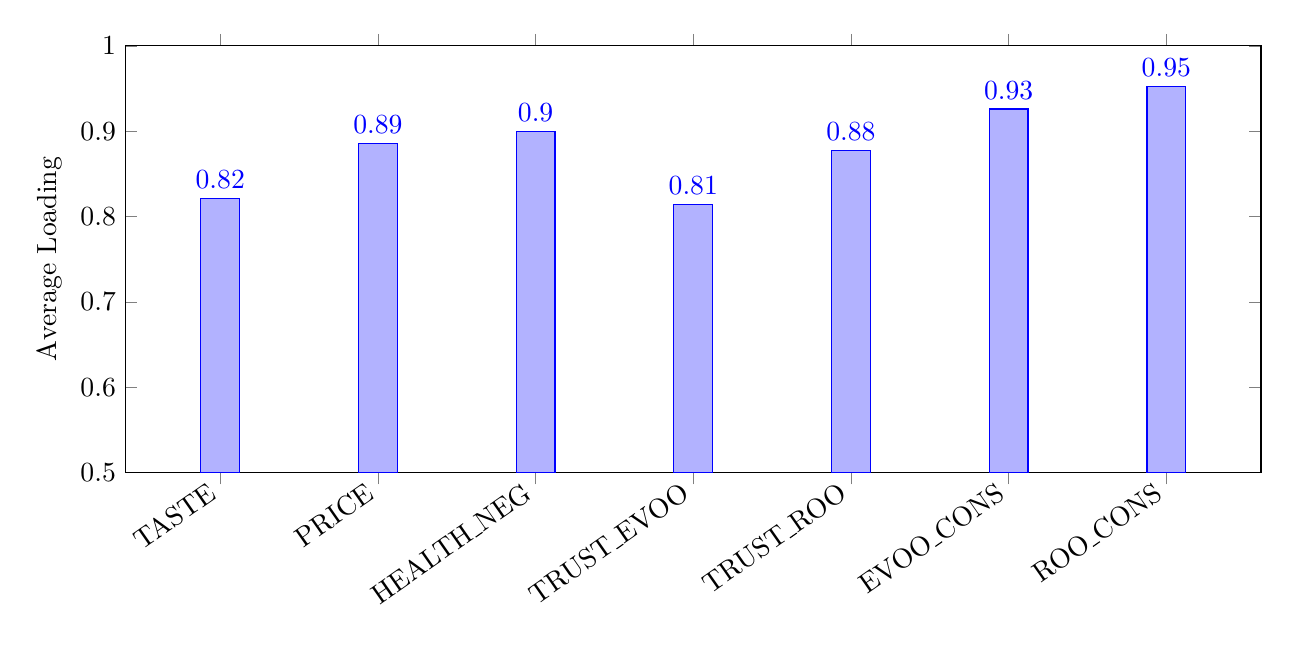
\begin{tikzpicture}
\begin{axis}[
    ybar,
    symbolic x coords={TASTE,PRICE,HEALTHNEG,TRUSTEVOO,TRUSTROO,EVOOCONS,ROOCONS},
    xtick=data,
    xticklabels={
        TASTE,
        PRICE,
        HEALTH\_NEG,
        TRUST\_EVOO,
        TRUST\_ROO,
        EVOO\_CONS,
        ROO\_CONS
    },
    xticklabel style={rotate=35, anchor=east},
    ymin=0.5, ymax=1.0,
    ylabel={Average Loading},
    width=16cm,
    height=7cm,
    bar width=14pt,
    nodes near coords,
    nodes near coords align={vertical},
]
\addplot coordinates {
    (TASTE,0.821)
    (PRICE,0.886)
    (HEALTHNEG,0.900)
    (TRUSTEVOO,0.814)
    (TRUSTROO,0.877)
    (EVOOCONS,0.926)
    (ROOCONS,0.952)
};
\end{axis}
\end{tikzpicture}
\caption{Average standardized indicator loadings for each reflective construct.}
\end{figure}



\begin{figure}[H]
\centering
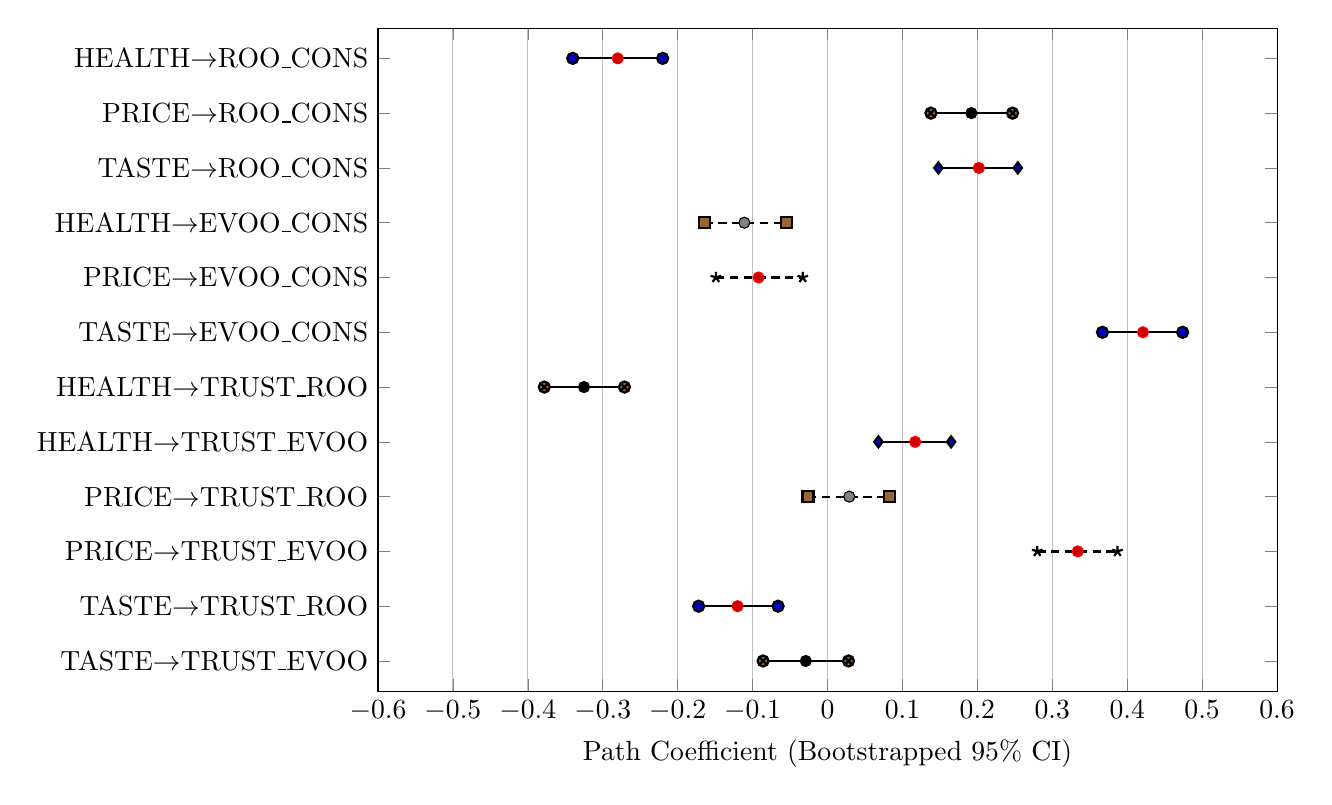
\begin{tikzpicture}
\begin{axis}[
    xshift=0cm,
    width=13cm,
    height=10cm,
    xmajorgrids,
    xmin=-0.6, xmax=0.6,
    xlabel={Path Coefficient (Bootstrapped 95\% CI)},
    ytick={
        1,...,12
    },
    yticklabels={
        TASTE$\rightarrow$TRUST\_EVOO,
        TASTE$\rightarrow$TRUST\_ROO,
        PRICE$\rightarrow$TRUST\_EVOO,
        PRICE$\rightarrow$TRUST\_ROO,
        HEALTH$\rightarrow$TRUST\_EVOO,
        HEALTH$\rightarrow$TRUST\_ROO,
        TASTE$\rightarrow$EVOO\_CONS,
        PRICE$\rightarrow$EVOO\_CONS,
        HEALTH$\rightarrow$EVOO\_CONS,
        TASTE$\rightarrow$ROO\_CONS,
        PRICE$\rightarrow$ROO\_CONS,
        HEALTH$\rightarrow$ROO\_CONS
    },
    enlarge y limits=0.05
]

% Example CI + point estimates:
% Each \addplot is: (lowerCI, y) -- (upperCI, y)
% Then \addplot[mark=*] places the point.

\addplot+[black, thick] coordinates {(-0.340,12) (-0.220,12)};
\addplot+[only marks,mark=*] coordinates {(-0.280,12)};

\addplot+[black, thick] coordinates {(0.138,11) (0.247,11)};
\addplot+[only marks,mark=*] coordinates {(0.192,11)};

\addplot+[black, thick] coordinates {(0.148,10) (0.254,10)};
\addplot+[only marks,mark=*] coordinates {(0.202,10)};

\addplot+[black, thick] coordinates {(-0.164,9) (-0.055,9)};
\addplot+[only marks,mark=*] coordinates {(-0.111,9)};

\addplot+[black, thick] coordinates {(-0.149,8) (-0.033,8)};
\addplot+[only marks,mark=*] coordinates {(-0.092,8)};

\addplot+[black, thick] coordinates {(0.367,7) (0.474,7)};
\addplot+[only marks,mark=*] coordinates {(0.421,7)};

\addplot+[black, thick] coordinates {(-0.378,6) (-0.271,6)};
\addplot+[only marks,mark=*] coordinates {(-0.325,6)};

\addplot+[black, thick] coordinates {(0.068,5) (0.165,5)};
\addplot+[only marks,mark=*] coordinates {(0.117,5)};

\addplot+[black, thick] coordinates {(-0.026,4) (0.083,4)};
\addplot+[only marks,mark=*] coordinates {(0.029,4)};

\addplot+[black, thick] coordinates {(0.280,3) (0.387,3)};
\addplot+[only marks,mark=*] coordinates {(0.334,3)};

\addplot+[black, thick] coordinates {(-0.172,2) (-0.066,2)};
\addplot+[only marks,mark=*] coordinates {(-0.120,2)};

\addplot+[black, thick] coordinates {(-0.086,1) (0.028,1)};
\addplot+[only marks,mark=*] coordinates {(-0.029,1)};

\end{axis}
\end{tikzpicture}
\caption{Forest plot of structural path estimates with 95\% bootstrap CIs.}
\end{figure}

\begin{figure}[H]
\centering
\includegraphics[width=0.95\textwidth]{appendix/total_effects.png}
\caption{Total effects (direct + mediated) from key perceptions to EVOO and ROO consumption.}
\end{figure}

\begin{table}[H]
\centering
\caption{Bootstrapped Total Effects (Direct + Indirect)}
\begin{tabular}{lrrrr}
\toprule
\textbf{Total Effect} & \textbf{Est.} & \textbf{Mean} & \textbf{SD} & \textbf{95\% CI} \\
\midrule
TASTE $\rightarrow$ EVOO\_CONS  & -0.471 & -0.471 & 0.027 & [-0.523, -0.416] \\
TASTE $\rightarrow$ ROO\_CONS   & 0.454 & 0.453 & 0.026 & [0.401, 0.504] \\
PRICE $\rightarrow$ EVOO\_CONS  & 0.215 & 0.215 & 0.026 & [0.165, 0.267] \\
PRICE $\rightarrow$ ROO\_CONS   & -0.198 & -0.198 & 0.027 & [-0.250, -0.145] \\
HEALTH\_NEG $\rightarrow$ EVOO\_CONS & -0.117 & -0.117 & 0.029 & [-0.175, -0.059] \\
HEALTH\_NEG $\rightarrow$ ROO\_CONS  & 0.119 & 0.119 & 0.028 & [0.064, 0.173] \\
TRUST\_EVOO $\rightarrow$ ROO\_CONS & -0.221 & -0.222 & 0.030 & [-0.281, -0.161] \\
TRUST\_ROO $\rightarrow$ EVOO\_CONS & -0.273 & -0.273 & 0.024 & [-0.320, -0.226] \\
\bottomrule
\end{tabular}
\end{table}

\begin{table}[H]
\centering
\caption{Measurement Model: Loadings, Reliability, and AVE}
\begin{tabular}{lcccc}
\toprule
\textbf{Construct} & \textbf{Indicator} & \textbf{Loading} & \textbf{CR (rhoC)} & \textbf{AVE} \\
\midrule
TASTE & taste\_1 & 0.804 & \multirow{3}{*}{0.862} & \multirow{3}{*}{0.675} \\
      & taste\_2 & 0.788 & & \\
      & taste\_3 & 0.871 & & \\
\midrule
PRICE & price\_1 & 0.933 & \multirow{2}{*}{0.881} & \multirow{2}{*}{0.787} \\
      & price\_3 & 0.839 & & \\
\midrule
HEALTH\_NEG & neg\_con\_1 & 0.909 & \multirow{2}{*}{0.895} & \multirow{2}{*}{0.811} \\
            & neg\_con\_3 & 0.891 & & \\
\midrule
TRUST\_EVOO & act\_evoo\_1 & 0.746 & \multirow{4}{*}{0.888} & \multirow{4}{*}{0.664} \\
            & act\_evoo\_2 & 0.838 & & \\
            & act\_evoo\_3 & 0.859 & & \\
            & act\_evoo\_4 & 0.812 & & \\
\midrule
TRUST\_ROO & act\_roo\_1 & 0.872 & \multirow{4}{*}{0.930} & \multirow{4}{*}{0.768} \\
           & act\_roo\_2 & 0.869 & & \\
           & act\_roo\_3 & 0.886 & & \\
           & act\_roo\_4 & 0.881 & & \\
\midrule
EVOO\_CONS & evoo\_con  & 0.928 & \multirow{2}{*}{0.923} & \multirow{2}{*}{0.856} \\
           & evoo\_uses & 0.923 & & \\
\midrule
ROO\_CONS & roo\_con  & 0.954 & \multirow{2}{*}{0.951} & \multirow{2}{*}{0.906} \\
          & roo\_uses & 0.950 & & \\
\bottomrule
\end{tabular}
\end{table}

\begin{table}[H]
\centering
\caption{Bootstrapped Structural Paths (5,000 resamples)}
\begin{tabular}{lrrrrr}
\toprule
\textbf{Path} & \textbf{Est.} & \textbf{Mean} & \textbf{SD} & \textbf{t-value} & \textbf{95\% CI} \\
\midrule
TASTE $\rightarrow$ TRUST\_EVOO & -0.280 & -0.281 & 0.031 & -9.18 & [-0.340, -0.220] \\
TASTE $\rightarrow$ TRUST\_ROO  & 0.192 & 0.192 & 0.028 & 6.86 & [0.138, 0.247] \\
TASTE $\rightarrow$ EVOO\_CONS  & -0.325 & -0.325 & 0.027 & -12.05 & [-0.378, -0.271] \\
TASTE $\rightarrow$ ROO\_CONS   & 0.334 & 0.333 & 0.027 & 12.31 & [0.280, 0.387] \\
\midrule
PRICE $\rightarrow$ TRUST\_EVOO & 0.202 & 0.202 & 0.028 & 7.30 & [0.148, 0.254] \\
PRICE $\rightarrow$ TRUST\_ROO  & -0.111 & -0.111 & 0.028 & -3.96 & [-0.164, -0.055] \\
PRICE $\rightarrow$ EVOO\_CONS  & 0.117 & 0.117 & 0.025 & 4.69 & [0.068, 0.165] \\
PRICE $\rightarrow$ ROO\_CONS   & -0.120 & -0.120 & 0.026 & -4.54 & [-0.172, -0.066] \\
\midrule
HEALTH\_NEG $\rightarrow$ TRUST\_EVOO & -0.092 & -0.092 & 0.030 & -3.10 & [-0.149, -0.033] \\
HEALTH\_NEG $\rightarrow$ TRUST\_ROO  & 0.421 & 0.421 & 0.028 & 15.27 & [0.367, 0.474] \\
HEALTH\_NEG $\rightarrow$ EVOO\_CONS  & 0.029 & 0.029 & 0.028 & 1.05 & [-0.026, 0.083] \\
HEALTH\_NEG $\rightarrow$ ROO\_CONS   & -0.029 & -0.028 & 0.029 & -1.00 & [-0.086, 0.028] \\
\midrule
TRUST\_EVOO $\rightarrow$ EVOO\_CONS & 0.334 & 0.334 & 0.027 & 12.45 & [0.281, 0.386] \\
TRUST\_EVOO $\rightarrow$ ROO\_CONS & -0.221 & -0.222 & 0.030 & -7.28 & [-0.281, -0.161] \\
TRUST\_ROO $\rightarrow$ EVOO\_CONS & -0.273 & -0.273 & 0.024 & -11.22 & [-0.320, -0.226] \\
TRUST\_ROO $\rightarrow$ ROO\_CONS & 0.302 & 0.302 & 0.025 & 12.31 & [0.254, 0.350] \\
\bottomrule
\end{tabular}
\end{table}


\begin{table}[H]
\centering
\caption{HTMT Discriminant Validity}
\begin{tabular}{lrrrr}
\toprule
\textbf{Construct Pair} & \textbf{HTMT} & \textbf{Mean} & \textbf{SD} & \textbf{95\% CI} \\
\midrule
TASTE -- PRICE & 0.093 & 0.100 & 0.037 & [0.039, 0.181] \\
TASTE -- HEALTH\_NEG & 0.515 & 0.515 & 0.037 & [0.439, 0.588] \\
TASTE -- TRUST\_EVOO & 0.411 & 0.410 & 0.035 & [0.340, 0.479] \\
TASTE -- TRUST\_ROO  & 0.439 & 0.439 & 0.031 & [0.378, 0.500] \\
TASTE -- EVOO\_CONS  & 0.669 & 0.669 & 0.029 & [0.612, 0.724] \\
TASTE -- ROO\_CONS   & 0.624 & 0.624 & 0.028 & [0.567, 0.677] \\
PRICE -- HEALTH\_NEG & 0.048 & 0.070 & 0.027 & [0.025, 0.134] \\
PRICE -- TRUST\_EVOO & 0.271 & 0.271 & 0.034 & [0.203, 0.336] \\
PRICE -- TRUST\_ROO  & 0.136 & 0.136 & 0.039 & [0.061, 0.213] \\
PRICE -- EVOO\_CONS  & 0.301 & 0.301 & 0.038 & [0.226, 0.374] \\
PRICE -- ROO\_CONS   & 0.272 & 0.272 & 0.037 & [0.197, 0.344] \\
HEALTH\_NEG -- TRUST\_EVOO & 0.243 & 0.242 & 0.037 & [0.169, 0.314] \\
HEALTH\_NEG -- TRUST\_ROO  & 0.593 & 0.593 & 0.027 & [0.539, 0.646] \\
HEALTH\_NEG -- EVOO\_CONS  & 0.369 & 0.370 & 0.037 & [0.296, 0.442] \\
HEALTH\_NEG -- ROO\_CONS   & 0.350 & 0.350 & 0.035 & [0.283, 0.418] \\
TRUST\_EVOO -- TRUST\_ROO  & 0.093 & 0.100 & 0.012 & [0.077, 0.127] \\
TRUST\_EVOO -- EVOO\_CONS  & 0.557 & 0.557 & 0.031 & [0.498, 0.615] \\
TRUST\_EVOO -- ROO\_CONS   & 0.412 & 0.412 & 0.035 & [0.342, 0.480] \\
TRUST\_ROO -- EVOO\_CONS   & 0.460 & 0.460 & 0.026 & [0.411, 0.510] \\
TRUST\_ROO -- ROO\_CONS    & 0.476 & 0.476 & 0.023 & [0.432, 0.520] \\
EVOO\_CONS -- ROO\_CONS    & 0.985 & 0.986 & 0.010 & [0.966, 1.005] \\
\bottomrule
\end{tabular}
\end{table}




\subsection{Multi-Group Analysis (MGA)}
To assess heterogeneity, we conduct MGA by estimating models within predefined groups (e.g., income tertiles, frequent vs.\ infrequent users, age groups) and testing differences in key effects or importances. For GLMs, we compare coefficients across groups using bootstrap standard errors and permutation tests on cross-validated losses. For RF, we compare group-specific permutation importances and PD/ALE shapes. Formally, for a parameter/importance $\theta^{(g)}$ in group $g$, we test
\begin{equation}
H_0: \theta^{(g_1)} = \theta^{(g_2)} \quad \text{vs.} \quad H_A: \theta^{(g_1)} \neq \theta^{(g_2)},
\end{equation}
using a null distribution from label permutations or pooled bootstrap resampling.

Compare key effects/importances across subgroups. Example: Quality perception is more predictive among high-income households (importance difference $=0.07$, perm.\ $p=0.02$), whereas price sensitivity dominates for low-income groups. Provide a table of group-specific metrics and a plot of PD curves by group.
% Optional: mention PD/ALE figures in Appendix.

\end{document}
